%%%%%%%%%%%%%%%%%%%%%%%%%%%%%%%%%%%%
% This is the template for submission to HPCA 2019
% The cls file is a modified from  'sig-alternate.cls'
%%%%%%%%%%%%%%%%%%%%%%%%%%%%%%%%%%%%

\documentclass{sig-alternate}
\setlength{\paperheight}{11in}
\setlength{\paperwidth}{8.5in}

\newcommand{\ignore}[1]{}
\usepackage[pass]{geometry}
\usepackage{fancyhdr}
\usepackage[normalem]{ulem}
\usepackage[hyphens]{url}
\usepackage{hyperref}
\usepackage{color}
\usepackage{soul}

\usepackage{amsmath}
\usepackage{amssymb}
\usepackage{tabularx}
\usepackage{setspace}

\usepackage{cite}

\usepackage[justification=centering]{caption}

\usepackage{microtype}

%\ifCLASSINFOpdf
%   \usepackage[pdftex]{graphicx}
%\else
% \usepackage[dvips]{graphicx}
%\fi
  % declare the path(s) where your graphic files are
  % \graphicspath{{../pdf/}{../jpeg/}}
  % and their extensions so you won't have to specify these with
  % every instance of \includegraphics
  % \DeclareGraphicsExtensions{.pdf,.jpeg,.png}
  % or other class option (dvipsone, dvipdf, if not using dvips). graphicx
  % will default to the driver specified in the system graphics.cfg if no
  % driver is specified.
 %\usepackage[dvips]{graphicx}
  % declare the path(s) where your graphic files are
  % \graphicspath{{../eps/}}
  % and their extensions so you won't have to specify these with
  % every instance of \includegraphics
  % \DeclareGraphicsExtensions{.eps}
%\ifCLASSOPTIONcompsoc
  \usepackage[caption=false,font=normalsize,labelfont=sf,textfont=sf]{subfig}
%\else
 % \usepackage[caption=false,font=footnotesize]{subfig}
%\fi


\usepackage{float}

\usepackage{amsmath}

\usepackage{fancyhdr}
\usepackage{hyperref}

%%%%%%%%%%%---SETME-----%%%%%%%%%%%%%
\newcommand{\hpcasubmissionnumber}{XXX}
%%%%%%%%%%%%%%%%%%%%%%%%%%%%%%%%%%%%
%\sethlcolor{white}

% When sethlcolor is white, your highlights will not show up.  Use
% \sethlcolor{white} to submit your paper pdf.  When compiling your second
% pdf with highlighted changes, simply remove \sethlcolor{white} and add your
% optional 100-word appendix.
% Use \hl{ ... } to highlight any text.
%%%%%%%%%%%%%%%%%%%%%%%%%%%%%%%%%%%%

\fancypagestyle{firstpage}{
  \fancyhf{}
\setlength{\headheight}{50pt}
\renewcommand{\headrulewidth}{0pt}
  \fancyhead[C]{\normalsize{HPCA 2019 Submission
      \textbf{\#\hpcasubmissionnumber} -- Confidential Draft -- Do NOT Distribute!!}}
  \pagenumbering{arabic}
}

%%%%%%%%%%%---SETME-----%%%%%%%%%%%%%
\title{Energy-efficient Adaptive Checkpoint Schemes for Computational Error Tolerant System}
%%%%%%%%%%%%%%%%%%%%%%%%%%%%%%%%%%%%

\begin{document}
\sloppy
\maketitle
\thispagestyle{firstpage}
\pagestyle{plain}



%%%%%% -- PAPER CONTENT STARTS-- %%%%%%%%

\begin{abstract}

Denard scaling has end. Because of the leakage current, system energy saving via lower supply voltage is no longer feasible in traditional device, e.g. MOSFETs. Some recent proposed techniques should be able to mitigate this problem due to they can keep a high on/off ratio of drain currents in a much lower supply voltage. But the major constraint of the new technologies is they may suffer intermittent errors in high probability which finally leads system to crash. Computational error correction architectures aim to tolerate these errors and enable Denard scaling further extended. However, the energy saving abilities are restricted in current architectures due to they at most can tolerate only one error, which significantly limits the potential of further supply voltage turn down. 

In this paper we exploit the error detection and correction properties of Redundant Residue Number System(RRNS). By carefully choose the RRNS base sets, our new architecture significantly improve the error tolerant ability which could detect all of the double residue errors and part of three or more residue errors. And we can safely remove the large size error correction table exists in RRNS error correction systems. Moreover, we design two energy-efficient adaptive checkpoint and rollback schemes: Extra Overhead Estimations and Error Interval Heuristics. Both of them are trying to make the best tradeoff between the EDP and reliability by automatically adjusting the long checkpoint intervals and incremental checkpoint intervals. On average, our new architecture with adaptive checkpoint scheme reduces 31.79\%  in energy consumption and 31.1\% in EDP when comparing with the previous single error correction architecture. Provide more energy saving opportunities via lowing the Vdd. 

\end{abstract}


\section{Introduction}
% no \IEEEPARstart

Dennard scaling was lost a decade ago due to ignoring the consideration of leakage current and threshold voltage limitation. The leakage current and threshold voltage does not scale but generating contributions to the power consumption per transistor. So power density soars with dimension decreasing and finally it hits the power wall.

Landauer\cite{Landauer_mini} proposed the minimum energy dissipation is usually on the order of `kT' for each of irreversible logic operation. The `k' represents the Boltzmann's constant and `T' is absolute temperature. So at room temperature, the value of `kT' is roughly equals to $4\times10^{-21}$ joules. Complementary Metal-Oxide Semiconductor (CMOS) can never reach this minimum threshold.  
CMOS is the most popular MOSFET technology today and widely used in current commercial products such as memories, ASICs, microprocessors and other digital logic circuits. However, the simple CMOS charging circuit constrains the energy reduction at Landauer-Shannon limit\cite{Landauer-Shannon}, which is about 50X higher than the minimal value proposed by Landauer.

Some new devices, such as Tunnel FETs\cite{TFET}, could operate below the limits of MOSFET devices. MOSFETs are limited to ln(10) kT/q $\approx$ 60 mV/decade sub threshold slope. These new devices are known as millivolt switches. However, just like the signal strength of a cell phone would become weaker as it moves further from the transmitter tower, the error rate of millivolt switches increase with an expression like $P_{e} = exp(-E_{signal} / kT)$ \cite{Agarwal}. So we must incorporate redundancy and error correction in logic or architecture design to keep the system error rate in bounds. In other words, if scaling continues with these devices go into production and some efficient error detection and/or correction schemes are proposed, technology should be able to go further to make the transistor signal energy between Landauer-Shannon limit and Landauer-Minimal. 

\subsection{Computational error detection and correction}
Standard error correcting codes (ECC)\cite{macwilliams1977theory}  is the most common error detection and correction code and widely adopted in modern communication or storage systems. However, ECC fails to protect the reliability from computational logics. For the upcoming new millivolt switch devices with higher error probability which work in low signal energy environment, we should design a computational error detectable architecture with minimal error diffusion probability.
\subsubsection{Triple Modular Redundancy(TMR)}
The conventional scheme for computational fault tolerance is called Triple Modular Redundancy(TMR)\cite{von1956probabilistic}. 
The basic idea of TMR is to duplicate the computational logic twice and then make a majority vote. If one of the computational logic is in error while remaining two are correct, this error could be simply corrected via the error-free majority voter.  However, TMR needs more than 200\% overhead in both area and power to detect and correct a single error. Any energy savings from lowering Vdd would be eclipsed due to this inefficient design. 

\subsubsection{Residue Checking}
Residue checking is another popular scheme widely used in IBM commercial processors, such as z990, z10, z196, POWER6 and POWER7\cite{ResidueCheck2011,IBMzEnterprise2011,Power6,Power7}. But it at least contains the following 4 constrains if used by upcoming millivolt switches: 
(1) Lower error detection coverage or higher checking overhead when comparing with Redundant Residue Number System(RRNS), which will be introduced in Section \ref{sub:RRNS}. Most IBM processors use very small moduli( e.g. 3, 9 or 15) so as to reduce the module complexity, but on the other hand these small numbers hurt the system error detection coverage(e.g. modulus 3, 1/3 errors are undetectable). Because the transient fault ratio should be much higher in near-threshold voltage, the system MTBF significantly goes down if adopting the residue checking method with these mini moduli. Increasing the modulus to a large number(e.g. 251*509) is necessary to reach the reasonable error detection capability. However the side-effect of using a large modulus is increasing the module logic complexity in both area and energy consumption, leading the overhead of a single residue checking is much worse than a single RRNS verification. 
(2) Residue Checking is necessary after every arithmetic operation.
If we don't perform residue check after a given arithmetic operation, then an error in that operation goes undetected forever. However, with RRNS, you can perform the RRNS checking at any time because the verification information remain exist in redundant residues.
3) The input data should be verified (e.g. ECC checking) before arithmetic computation.
If one of the inputs is in error, this residue checking circuit is unable to detect it. The residue checking can only detect the error generated during the ALU operations. However, the input checking is unnecessary in RRNS. 
4) Unable to optimize the ALU because the data are in binary format. If the data are in RRNS format, Index-sum algorithm\cite{DengTACO18} could be used to simplify the multiplier in ALU. However, the data in residue checking are in binary format. Binary data are not suitable to use the Index-sum method because the related LUT size would be pretty huge. \newline
One possible advantage of residue checking is it may get some latency benefits from a single check. The IBM residue checking operation at least takes 3 cycles while the cost of RRNS check is at most 8 cycles. But in the low energy system design, the latency isn't the first consideration. Moreover, both residue checking and RRNS checking latencies could be hided because none of them is in the critical path. 


\subsubsection{RNS and RRNS}
\label{sub:RRNS}
Residue Number Systems (RNS) has been extensively studied and used in digital signal processing (DSP), digital communication systems and cryptographic hardware. It works as an alternative to the binary number system. In RNS,  A large binary integer could be injectively mapped to a set of smaller integers and cases of parallelism and fault tolerant computation because of its carry-free property \cite{EricDSR,AndersonThesis}. Some of the RRNS properties are summarized below.

Let $B=\{m_i\in \mathbb{N}~for~i = 1,2,3,...,n\}$ be a set of $n$ pairwise relatively prime natural numbers, which we shall refer to as bases or moduli. $M=\prod_{i=1}^{n}m_i$ defines the range of natural numbers that can be injectively represented by RNS that is defined by the set of bases $B$. Specifically, for $x$ such that $x\in\mathbb{N}~and ~x < M$, then, $x \equiv (|x|_{m_1}, |x|_{m_2}, |x|_{m_3}, ..., |x|_{m_n})$, where $|x|_m = x~mod~m$. Each element in this $n$-tuple is referred to as a residue.The addition, subtraction, and multiplication of RNS can be performed independently and in parallel on the various residue. Given $x, y \in \mathbb{N}~and ~x, y < M$, we have $|x~op~y|_m=||x|_m~op~|y|_m|_m$, where $op$ is any add/subtract/multiply operation. This property could significant improve the performance and energy benefits, particularly for multiplication which is slow and expensive with conventional binary representation. However, the division of RNS need some specific high overhead algorithms\cite{RNSDivisionMansoureh,RNSDivisionTalahmeh}, so RNS architecture should avoid the division intensive workloads.

\begin{table*}
\centering{}
\footnotesize
\captionsetup{justification=centering}
\caption{\label{tab:RRNS}A (4, 2)-RRNS example with a toy base set (3, 5, 
2, 7, 11, 13). \newline 11 and 13 are the redundant bases. }
\begin{tabular}{|c|c|c|c|c|c|c|}
\hline 
Decimal & mod 3 & mod 5 & mod 2 & mod 7 & mod 11 & mod 13\tabularnewline
\hline 
\hline 
13 & 1 & 3 & 1 & 6 & 2 & 0\tabularnewline
\hline 
14 & 2 & 4 & 0 & 0 & 3 & 1\tabularnewline
\hline 
13+14=27 & (1+2)mod 3=0 & 2 & 1 & 6 & 5 & 1\tabularnewline
\hline 
 & \multicolumn{6}{c|}{All columns function independently of one another. }\tabularnewline
\cline{2-7} 
 & \multicolumn{6}{c|}{Any one of these columns in error can be corrected or  }\tabularnewline
 & \multicolumn{6}{c|}{any two in error can be detected by the remaining columns.}\tabularnewline

 
\hline 
\end{tabular}

\end{table*}


RNS can be easily extended with fault tolerance ability by adding $r$ redundant residues. The set of Redundant Residue Number Systems(RRNS) moduli contains $n$ non-redundant and $r$ redundant moduli: $B=\{m_i\in\mathbb{N}~for~i = 1,2,3,...,n,n+1,...,n+r\}$. Any integer number smaller than $M$ ($=\prod_{i=1}^{n}m_i$) can still be represented uniquely by its original $n$ non-redundant residues,so the additional  $r$residues are defined as redundant. For $x$ such that $x\in\mathbb{N},~x < M$, then, $x \equiv (|x|_{m_1}, |x|_{m_2}, |x|_{m_3}, ..., |x|_{m_n}, |x|_{m_{n+1}}, ..., |x|_{m_{n+r}})$ contains $n$ non-redundant residues as well as $r$ redundant residues. For convenience, we further define the redundant bases product as $M_R = \prod_{i=n+1}^{n+r}m_i$. 

One character of RRNS is residue error contained. Any arithmetic computation error that occurs in one of the residues is restricted in that residue and does not propagate to other residues. When it's necessary, the error can be detected and/or corrected with the help of the remaining residues. Specifically, an RRNS system with ($n$, $r$) = (4, 2), a single residue error can be corrected, or, two residues in error can be detected. Table \ref{tab:RRNS} provides a straightforward example with a toy moduli set to explain how RRNS works, Deng etc. \cite{DengTACO18} outlines necessary algorithms to do so. Research by Watson and Hastings  \cite{Hastings, WatsonThesis, WatsonHastings} proposed the foundation for the underlying theoretical algorithms. They used (199, 233, 194, 239, 251, 509) as the (4, 2)-RRNS system, providing a number system with range $M = 199\times 233\times 194\times 239 \in (2^{31}, 2^{32})$. Deng etc. \cite{DengTACO18} optimized the the RRNS multiplier and used (421,211,256,347,503,521) as the base set. The detailed conditions and considerations of RRNS base selection will be discussed in Section \ref{sub:RRNS bases}.

So RRNS is possible to gain significant benefit in designing an energy-efficient core because of carry-free bit-level parallelism and providing a low overhead error tolerated scheme with only around 50\% energy and area overhead. 

\subsection{CREEPY and limitations}
\label{sub:CREEPY}
Deng etc.\cite{DengICRC16,DengTACO18,SrikanthHPCA18} proposed a Single Error Correction(SEC) RRNS architecture with 4 non-redundant residues and 2 redundant residues, which is known as CREEPY or (4,2)-RRNS SEC. 
Actually (4,2)-RRNS configuration is able to correct single error residue or detect any of 2 error residues. However, the property of RRNS doesn't allow both capabilities to be supported simultaneously. In other words, only one of them can be selected at a time(CREEPY is SEC).  The reason is that the \textit{delta value pairs} from the output of RRNS checking algorithm may be overlapped in SEC and DED mechanism.  Figure \ref{fig_SECDED} gives an detailed example to explain this phenomenon. We use a simple toy (4,2)-RRNS base set (3,5,2,7,11,13) for easily computing. And the range of this toy set equals to $3 \times 5 \times 2 \times 7 = 210$, which is the product of all the non-redundant moduli while the 11 and 13 are redundant ones. In $1_{st}$ case, the original correct RRNS value is (0,3,0,0,3,12), and then the system gets one residue in error (the $1_{st}$ residue change from 0 to 2). If a RRNS check is inserted after this error, by using the Chinese Remainder Theorem\cite{goldreich1999chinese} or Base Extension Algorithm \cite{WatsonHastings,WatsonThesis}, the system gets a value pair ${m_{5}}^{'}$ and ${m_{6}}^{'}$. By making a modulus subtracting with the output of related redundant subcore respectively, finally the system gets the delta value pair $(\Delta m_{5}, \Delta m_{6})$. This delta value pair is an important output which directly relates to the RRNS residue error information. If both delta values equal to zero, it means that no error in this RRNS data; If only one of them doesn't equal to zero, the corresponding redundant core should be in error. The correction of this case is straightforward, we can use the output of Chinese Remainder Theorem or Base Extension Algorithm to replace the error redundant subcore. If both delta values don't equals to zero, it means the error is in one of the non-redundant subcore and we have to check the error correction table. In the example \textit{delta value pair} (5,9) is used as the input to search the table, and we found the entry with a related output (2,1). The output (2,1) means the system should add a correction factor \`1\` to the second non-redundant subcore to make the correction.  In this one error example, because  all the computation  in subcore 2 would automatically module 3, so this one residue error could be fixed by adding this correction factor. This mechanism works well if it only supports SEC. But if the system is SECDED, from the two error example of  Figure \ref{fig_SECDED}, we can finally get a same delta value pair $(\Delta m_{5}, \Delta m_{6})$. If checking the error correction table and adding the correction factor in this double error case, the output will be wrong.This two error detection should rollback to the previous valid checkpoint and re-execute. In other words, the system is unable to always make the right decision for correction or rollback if it supports SECDEC. So only one of the capability, SEC or DEC, could be used in (4,2)-RRNS system at a time.  

\begin{figure}[H]
\centering
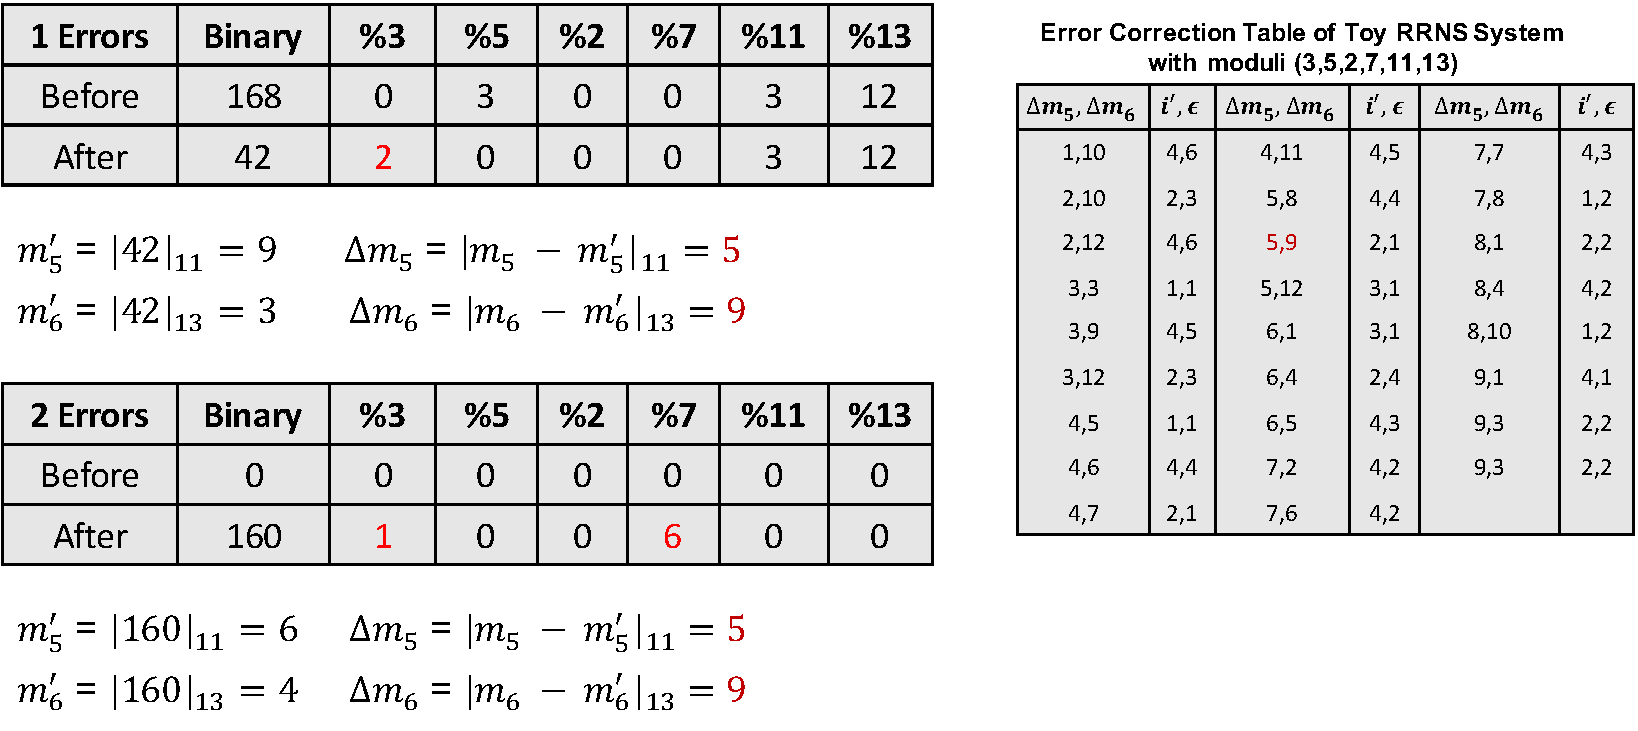
\includegraphics[width=3.5in]{graphics/SECorDED.pdf}

\caption{An Example of SECDED conflict in a same (4,2)-RRNS system}
\label{fig_SECDED}
\end{figure}

In CREEPY, two or more residues in error are defined as failure. But if (4,2)-RRNS DED with a checkpoint scheme is used, the system failure threshold could be upgraded to three or more residues in error. This gives the potential for the signal energy further turned down and get the energy benefit. Another possible option for error detection is to cut down one redundant residue and make it as (4,1)-RRNS Single Error Detection(SED). This may reduce each of computation and RRNS checking overhead, but lost reliability in theory. 

From the simulation result in Section \ref{Evaluation}, (Energy Delay Product)EDP can further reduce 31.1\% when comparing  with CREEPY if designing an efficient checkpoint and rollback mechanism with double error detection infrastructure. Moreover, CREEPY needs a large size error correction table which stored in ROM, which significantly increasing the hardware and area overhead. 

\subsection{Contributions}
\begin{enumerate}
\item Deisgn (4,1)-RRNS and (4,2)-RRNS checkpoint systems with reasonable base sets and supported efficient incremental checkpoint mechanism. 
\item Remove the ROM units which stored the large size error correction table. 
\item Proposed 2 adaptive checkpoint interval adjustment methods and the best scheme reducing 31.1\% of energy and EDP compared with CREEPY on average. 
\item Improve the feasibility of RRNS system. In  (4,2)-RRNS DED configuration, the related error model could tolerate at most two errors between two checks. But in CREEPY, it only allows one error between two checks. 
\end{enumerate}
% You must have at least 2 lines in the paragraph with the drop letter
% (should never be an issue)

%\subsection{Format Highlights}
%\begin{itemize}
%\item Paper must be submitted in printable PDF format.
%\item Text must be in a minimum 10pt font, see Table~\ref{table:formatting}.
%\item Papers must be at most 11 pages, not including references.
%\item No page limit for references.
%\item Each reference must specify {\em all} authors (no {\em et al.}).
%\item Authors of {\em all} accepted papers will be required to give a
%lightning presentation (about 90s) and a poster in addition to the regular
%conference talk.
%\end{itemize}



%------------------------------------------------
\section{RRNS Checkpoint System Architecture}

\begin{figure*}[!t]
\centering
\subfloat[(4,1)-RRNS Single Error Detection(SED) Core]{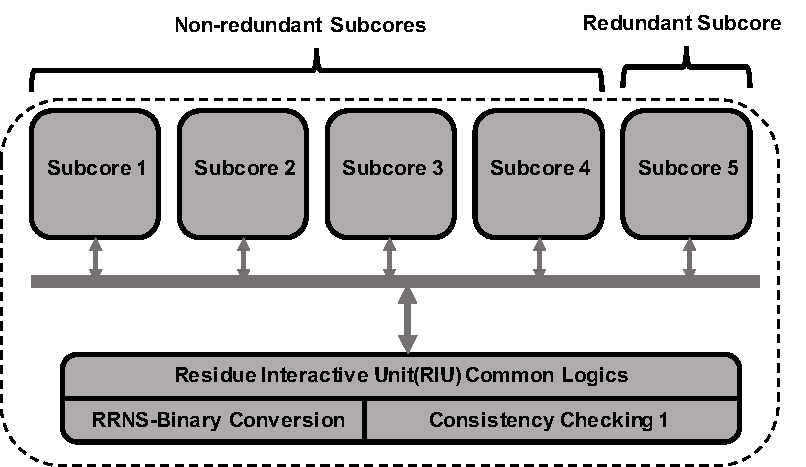
\includegraphics[width=3.05in]{graphics/41architecture.pdf}%
\label{fig_arch_41}}
\hfil
\subfloat[(4,2)-RRNS Double Error Detection(DED) Core]{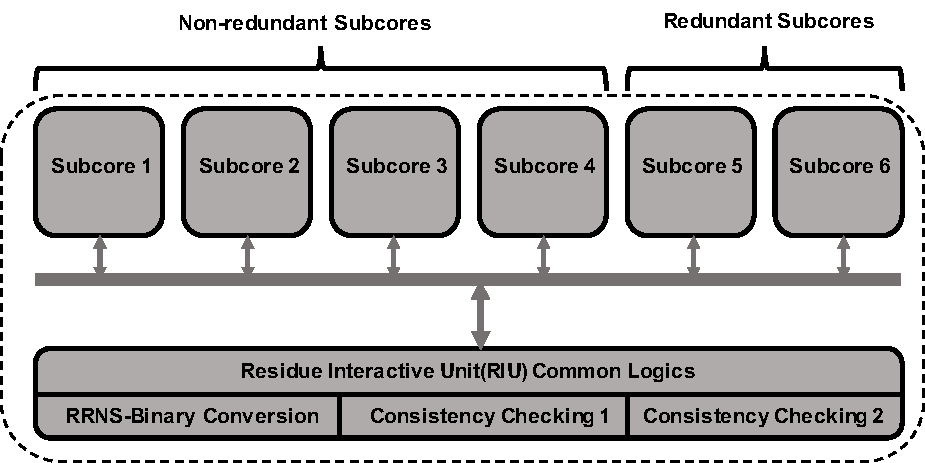
\includegraphics[width=3.5in]{graphics/42architecture.pdf}%
\label{fig_arch_42}}
\caption{RRNS Checkpoint and Rollback Core Overview}
\label{fig_arch}
\end{figure*}

As discussed in Section \ref{sub:CREEPY}, we have two possible solutions to further reduce the energy consumption when comparing with CREEPY: (4,1)-RRNS Single Error Detection (SED) and (4,2)-RRNS Double Error Detection (DED). Because lack of error correction ability in these two configurations, designing an efficient error detection and rollback mechanism is necessary for the recovery from error or failure. More details about the adaptive checkpoint and rollback schemes will be discussed in Section \ref{Chptschemes}. 

Figure \ref{fig_arch} shows the architecture overview of the two possible RRNS Checkpoint and Rollback Systems. Each RRNS core includes 4 non-redundant subcores and 1 or 2 redundant subcores. The Instruction Register is shared by all the subcores and protected by ECC. Similar to CREEPY architecture, ICache is shared by all the subcore while Dcache is distributed in each of the subcore(each subcore only store one residue of the RRNS value). And the Memory could be protected via efficient ECC and assuming error free in this paper. 

The architecture of (4,2)-RRNS DED configuration is similar to CREEPY. The biggest difference is no large size error correction table in these checkpoint and rollback system. The Residue Interactive Unit(RIU) consists of RRNS-Binary Conversion Unit and Consistency Checking Unit. The number of Consistency Checking Unit depends on the amount of redundant subcore.  (4,2)-RRNS DED needs two Consistency Checking Units while 
 (4,2)-RRNS DED only needs one. Because of less dynamic energy consumption in each of the computation and in each of consistency checking,  (4,1)-RRNS SED may have the potential to get energy benefit even though it may loss some reliability. On average, one third of error in (4,1)-RRNS SED system is undetectable, and this undetectable error is also defined as one kind of failure. So the MTBF of (4,1)-RRNS SED system should be lower in a same signal energy level. In other words, we may need higher signal energy to keep the reliability at a same level. For the (4,2)-RRNS DED, because it can detect all the 1-residue or 2-residue errors and majority of multiple-errors if the RRNS base set is carefully selected, the MTBF should be higher at a same signal energy level. So signal energy of (4,2)-RRNS DED system could be further turned down and probably to save system energy if an efficient checkpoint mechanism is used. 

\subsection{Bases Selections for Both Systems}
\label{sub:RRNS bases}
The base sets used in the RRNS core depend on the number of redundant residues and the error detection/correction capability. E.g, in (4,2)-RRNS, the base set candidates should be different for single error correction(SEC) and double error detection(DEC).  The SEC base set options are discussed in CREEPY \cite{DengTACO18}. Because the RRNS checkpoint mechanism is based on the theory of DED, we list the necessary and sufficient conditions for (4,2)-RRNS double error detection here:
\begin{enumerate}
\item Each pair of bases $m_{i}$,$m_{j}$ must be relatively prime.
\item All the products of the 2 moduli taken 2-(2-j) at a time are greater than the maximum product of j N-R moduli, where j =1 or 2. 
\item $|m_{1}m_{2} - m_{3}m_{4}|$ = 1; also known as the K, K-1 property. (For RRNS fractional multiplication.)
\item mi $\in$ \{x $|$ x is either prime (p), a power of prime ($p^{m}$), or a power of 2 ($2^{m}$) \}. Recall that the relative order of preference is p $> p^{m} > 2^{m}$ , and that smaller bases result in smaller ROMs. (For index sum multiplication.) 
\end{enumerate}

The proof of these conditions are available in \cite{WatsonThesis}. Table \ref{tab:Bases} are the base set candidates of (4,2)-RRNS DED system. The total number of \textit{Core Bit}, \textit{Range} and \textit{Base Format} are there factors we should consider when choosing the bases. The \textit{Core Bit} directly relate to the area, hardware and energy overhead. For the \textit{Range}, larger is better. The \textit{Base Format} is related to the index-sum multiply algorithm \cite{DengTACO18} and the preference order is p $> p^{m} > 2^{m}$. The base set proposed by Waston\cite{WatsonThesis} and the range of 32-bit binary are added in the table for comparison purpose. If preferring low energy, less hardware and no large numbers in the applications, the base set (113,239,128,211,241,251) would be the best choice. If range is an important factor, (139,349,128,379,509,503) may be a good option. If you want the range better than 32-bit binary, it has to choose (211,421,256,347,509,503).  Actually, this base set is only 1 bit more than (139,349,128,379,509,503) in total \textit{Core Bit} while it gets more than 2 times of range increment. 

\begin{table*}[t]
%\begin{table}[H]
  \centering
  \captionsetup{justification=centering}
  \tiny
  \setlength{\tabcolsep}{3pt}
\caption{\label{tab:Bases}Possible (4,2)-RRNS Base Sets}
  \begin{tabular}{|c|c|c|c|c|}
\hline 
\textbf{Subcore Bits} & \textbf{Core Bit}  & \textbf{Range} & \textbf{Possible Base Sets} & \textbf{Base Format}\tabularnewline
\hline 
$7,8,7,8,8,8$ & 46 & 467921792 &(97,223,128,169,241,251)&$(p,p,2^7, 13^2,p,p)$\tabularnewline
\hline 
$7,8,7,8,8,8$ & 46 & 729405056 & \textbf{(113,239,128,211,241,251)} &$(p,p,2^7, p,p,p)$\tabularnewline
\hline 
$8,8,7,8,8,8$ & 47 & 635871872 & (151,167,128,197,241,251)&$(p,p,2^7, p,p,p)$\tabularnewline
\hline 
$7,8,8,7,9,9$ & 48 & 430002432 & (89,233,256,81,509,503)&$(p,p,2^8, 3^4,p,p)$\tabularnewline
\hline 
$7,9,7,8,9,9$ & 49 & 951568256 & (109,283,128,241,509,503)&$(p,p,2^7, p,p,p)$\tabularnewline
\hline 
$7,9,7,8,9,9$ & 49 & 1032240512 & (89,361,128,251,509,503)&$(p,19^2,2^7, p,p,p)$\tabularnewline
\hline 
$8,8,8,8,8,9$ & 49& 2149852322&(199,233,194,239,251,509)&$Waston$\tabularnewline
\hline 
$9,7,7,9,9,9$ & 50& 1082179712&(491,67,128,257,509,503)&$(p,p,2^7, p,p,p)$\tabularnewline
\hline 
$7,9,7,9,9,9$ & 50& 1406512512&(81,463,128,293,509,503)&$(3^4,p,2^7, p,p,p)$\tabularnewline
\hline 
$7,9,8,8,9,9$ & 50& 1230080256&(81,433,256,137,509,503)&$(3^4,p,2^8,p,p,p)$\tabularnewline
\hline 
$8,9,7,9,9,9$ & 51& 2353365632&\textbf{(139,349,128,379,509,503)}&$(p,p,2^7, p,p,p)$\tabularnewline
\hline 
$ $ &  & 4294967296&& 32-bit binary\tabularnewline
\hline 
$8,9,8,9,9,9$ & 52& 7891035392&\textbf{(211,421,256,347,509,503)}&$(p,p,2^8,p,p,p)$\tabularnewline
\hline 
$9,9,8,9,9,9$ & 53& 7710332672&(277,317,256,343,509,503)&$(p,p,2^8,p^m,p,p)$\tabularnewline
\hline 
  \end{tabular}


\end{table*}
%\end{table}

Because (4,1)-RRNS system only includes one redundant residue, which means that it can detect a single residue in error. The necessary and sufficient conditions for (4,1)-RRNS single error detection actually is a subset of (4,2)-RRNS double error detection. Simply changing condition (2) of (4,2)-RRNS DED to ``The redundant modulus must be greater than the largest non-redundant residue``, we can get the limitations  for (4,1)-RRNS. Due to the space limitation, we don't list the (4,1)-RRNS base set candidates in the paper. 

\subsection{RRNS Checkpoint and Rollback Mechanism Overview}
\begin{figure}[H]
\centering
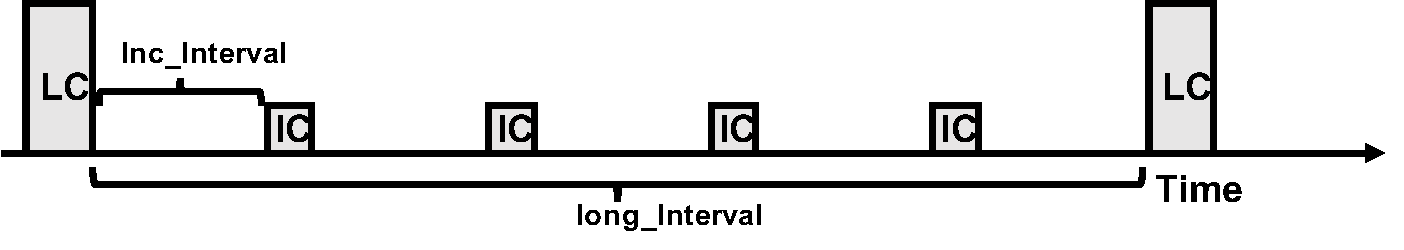
\includegraphics[width=3.5in]{graphics/chpt_overview.pdf}

\caption{RRNS Checkpoint Mechanism Flowchart}
\label{fig_chpt_overview}
\end{figure}

\begin{figure}[H]
\centering
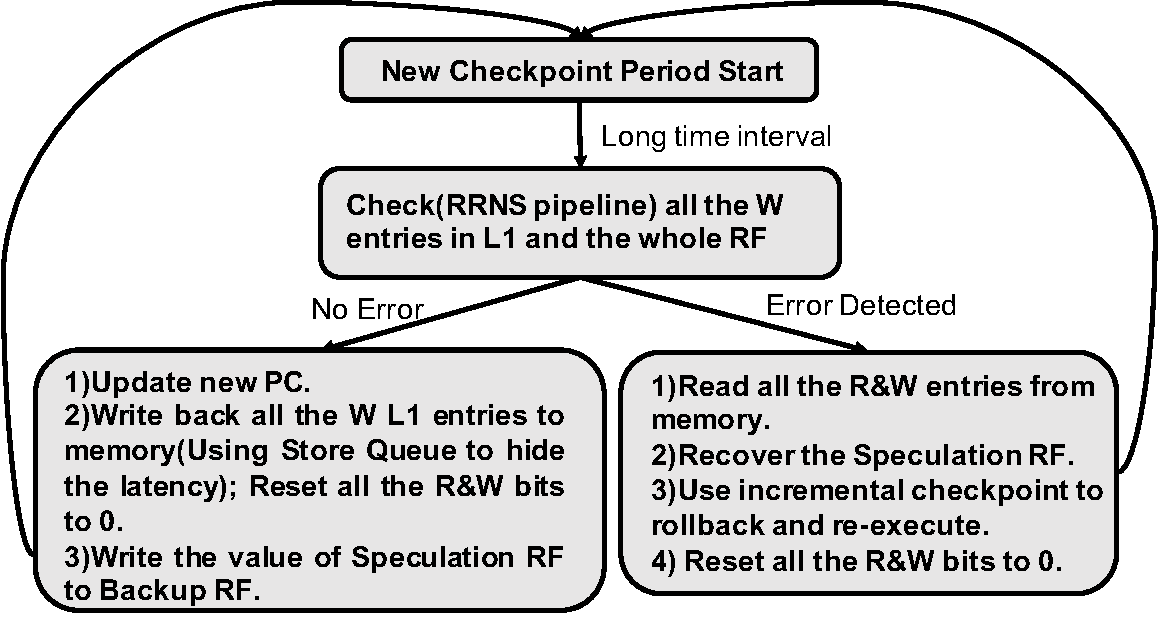
\includegraphics[width=3.5in]{graphics/chpt_flowchart.pdf}

\caption{RRNS Checkpoint Mechanism Overview With Incremental Checkpoints}
\label{fig_chpt_flowchart}
\end{figure}

Figure \ref{fig_chpt_overview} gives the overview about how RRNS checkpoint mechanism works with incremental checkpoint \cite{Naksinehaboon_incchpt, Agarwal_incchpt, Li_incchpt}. 
Right after \textit{Long\_Time\_Interval}, all the store values(extra queue) and destination register should be verified via RRNS checking algorithm. The \textit{Long\_Time\_Interval} may be fixed or variable, and it should be as long as possible while keeping good reliability. The \textit{Long\_Time\_Interval} could be divided into several \textit{Short\_Time\_Interval}(\textit{Incremental\_Interval}) and using incremental checkpoint to reduce the re-execution overhead. The overhead reduction depends on the error generation time and the number of incremental checkpoints in a long interval. More discussions about the incremental checkpoint are available in Section \ref{Inc_chpt}. After each of the \textit{Long\_Time\_Interval}, the system inserts  a Long Check(LC) to verify the correctness and update the system status, the details of LC operations are shown in Figure \ref{fig_chpt_flowchart}. In the current error model, we assume the memory is error free due to many protection techniques\ref{} are available. At the beginning of the LC, the system checks the whole Speculation RF and all the modified entries of cache(W entries) in pipeline way \cite{DengICRC16,DengTACO18} . It should be noted that we don't need to check the R cache entries. Because the load value and its related results would be immediately spread to Speculation RF or write back to Dcache. These values have to be verified later during LC phase. If no error is detected, we can simply update the PC, cache and Register File. But if one or more errors is detected, the system should recover to the previous verification status and then re-execution.  

The cache eviction behaviors become tricky in checkpoint mechanism and we can classify them into 3 cases: 
\begin{enumerate}
\item R==0 and W==0: The cache block can be directly evicted without any RRNS checking. Errors in this line won't affect the correctness pf result because nobody read it and it won't write back to the memory.  
\item R==1 and W==0: The cache block can be directly evicted without RRNS checking. Because these load errors would spread and be detected in RF or/and in `W' cache entries. Moreover, sometime the error may happen after the last usage. So we can directly ignore these errors because they won't affect the system correctness.  
\item W == 1: Need a RRNS check before eviction. If one or more errors is detected, rollback to the previous correct status; If no error is found, this line should be stored in a writeback buffer (It can't be written back to main memory immediately because this may change the current correct state of memory). Committing the writeback buffer to memory only after the whole checkpoint verification process completes.   
\end{enumerate}

\section{Adaptive Checkpoint and Rollback Schemes}

The value pair of \textit{Long\_Time\_Interval} and \textit{Incremental\_Interval} could significant affect the execution mode of the workload, such as the number of rollback back, the time of re-execution and etc. However, it's almost impossible to find out the best static long check intervals. Even the suboptimal static long check intervals vary in different application. So designing some efficient adaptive methods are necessary.

\subsection{Extra Overhead Estimation}
The long checkpoint interval is a critical factor for optimizing system energy and performance. In order to get the efficient tradeoff, It's necessary to figure out a reasonable checkpoint interval determination scheme. The scheme proposed in this section is called Extra Overhead Estimation(EOE). The basic idea of EOE is trying to estimate the next interval overhead based on the history information. Then making the decision of increasing, decreasing or keeping the old long check interval value. 

After the checkpoint verification procedure and no error detected, the system computes the following 3 fomulas:
\begin{equation}
\resizebox{.8\hsize}{!}{$All\_full+ All\_inc + \frac{\lfloor(1- \frac{E(X)}{Long\_Interval})\times num\_inc\rfloor +1}{num\_inc}\times ave\_long$}
\end{equation}
\begin{equation}
\resizebox{.8\hsize}{!}{$All\_full\times 0.5+ All\_inc + \frac{\lfloor(1- \frac{E(X)}{Long\_Interval})\times2\times num\_inc\rfloor +1}{num\_inc\times2}\times2\times ave\_long$}
\end{equation}
\begin{equation}
\resizebox{.8\hsize}{!}{$All\_full\times 2+ All\_inc + \frac{\lfloor(1- \frac{E(X)}{Long\_Interval})\times0.5\times num\_inc\rfloor +1}{num\_inc\times0.5}\times0.5\times ave\_long$}
\end{equation}

\begin{table}
\setlength{\abovecaptionskip}{-0.5pt}
\setlength{\belowcaptionskip}{-1pt}
\centering{}
\footnotesize
\captionsetup{justification=centering}
\caption{\label{tab:equation_expian}equation terminologies}

\begin{tabular}{|c|p{5cm}|}
\hline 
\textbf{Name} & \textbf{Explaination} \tabularnewline
\hline 
$All\_full $ & Overall full checkpoint verification and update overhead between the last 2 errors  \tabularnewline
\hline 
$All\_inc$ & Overall inc checkpoint creation overhead during the same time-slot \tabularnewline
\hline 
$E(X)$ & Expected value of error cycle in the last long checkpoint interval \tabularnewline
\hline 
$Long\_interval$ & The time interval between 2 full checks\tabularnewline
\hline 
$num\_inc$ & Number of incremental checkpoints in a single long checkpoint interval\tabularnewline
\hline 
$ave\_long$ & average overhead of long checkpoint interval between the last 2 errors\tabularnewline
\hline 

\end{tabular}
\vspace{-2mm}
\end{table}

The Formula (1) computes the total overhead between last 2 errors; The Formula (2) roughly estimates the total overhead if doubling the long time interval during the last 2 errors; Formula (3)  roughly estimates the total overhead if the halving the long time interval during the last 2 errors. The terminologies of these 3 formulas are explained in Table \ref{tab:equation_expian}. In order to compute the results of these formulas, we have to figure out the expected value of error time in the last long check interval. The details about how to compute the expected value E(X) are available in   APPENDIX \ref{appendix}. If Formula(1) gets the smallest value, the system keeps the long check interval value unchanged; If Formula(2) gets the smallest value, the system double the long check interval value; Similarly, If Formula(3) gets the smallest value, the system halves the long check interval value. 

\subsection{Error Interval Heuristics}
Error Interval Heuristics(EIH) mechanism is an empirical adaptive method. It's based on an assumption that the time intervals between 2 sequence errors should be similar in most cases. Based on this assumption, the probability of the error is detected in the first half time is lower, but the chance would increase as the time past. So we can insert less RRNS checks in the first half time and gradually increasing the check frequency in exponential way. Figure \ref{fig_adp_20} describes how the EIH works before the error is detected. In this example, we assume the last two errors interval is 200,000 cycles. In the $1^{st}$ iteration, long check interval is set to 200,000/2=100,000 cycles with no incremental checkpoint. Less check frequency is benefit from reducing system energy and performance loss. In the $2^{nd}$ iteration, system halves the old long check interval and insert one incremental checkpoint. Similarly, for the future iterations, we halve the last long check interval and double the number of incremental checkpoints. Minimal values for long interval and incremental interval are set because the overhead may exponentially increase if higher frequency long checks and/or incremental checks are used. In this example, we set the minimal long check interval to 30,000 cycles while the minimal incremental checkpoint interval is 10,000 cycles. So in iteration 3, the long interval is set to 30,000 instead of 25,000. For the iteration 4, the system keeps the old intervals due to both of them reach the limitations. In Figure \ref{fig_adp_20} would keep this checkpoint interval configuration until the $1^{st}$  error is detected. The system only performs RRNS checks at the end of current long interval (The L blocks in Figure \ref{fig_adp_2}), so it should always has a delay between error generation and error detection. 

Figure \ref{fig_adp_21} gives the details about how to handle the $1^{st}$  error. Once the  $1^{st}$  error is detected at the end of iteration 3, we should rollback to the last verified full system status (At the end of the$2^{nd}$ iteration), including PC, Register File and all the W cache blocks. Then checking the incremental checkpoints in sequential order. The  $1^{st}$  incremental checkpoint should be correct should write all the record data to the system. Similar checking the next incremental checkpoint until the error is detected. In this example the $2^{nd}$ incremental checkpoint is error and the system should re-execute from the status right after the $1^{st}$  incremental checkpoint. Set the new error interval value equals to summation cycles of these 3 iterations(100,000+50,000+30,000+checkpoint creating and RRNS verification time) and start a new execution process. 

We onIy discussion one error detection above. If two or more errors are found in a same long interval, this may imply high error probability and the system needs higher frequency check. So in this case, the error interval is set to the value of last long interval divided by number of errors. Then start the new execution. 

\begin{figure*}[!t]
\centering
\subfloat[No error is detected]{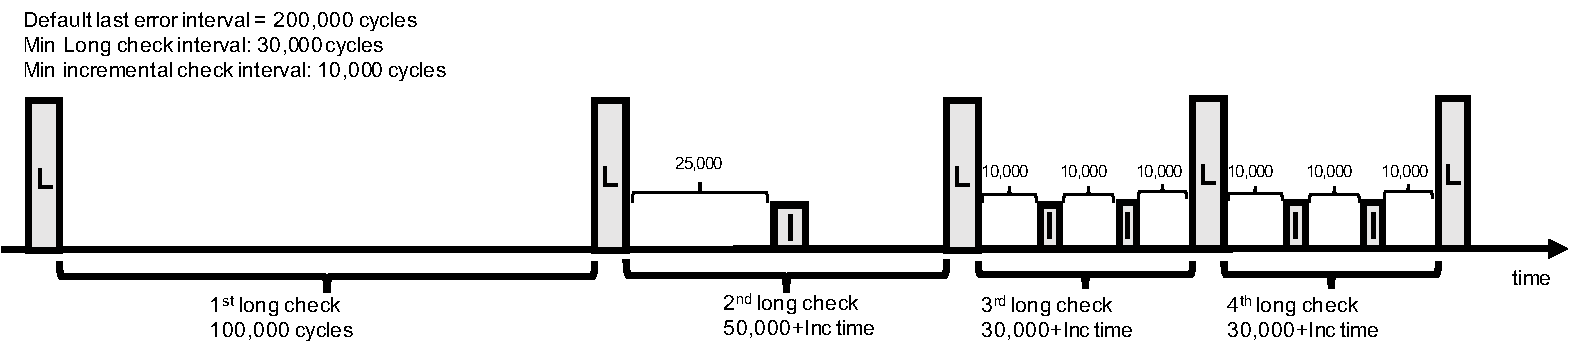
\includegraphics[width=3.3in]{graphics/adaptive2.pdf}%
\label{fig_adp_20}}
\hfil
\subfloat[An error is detected]{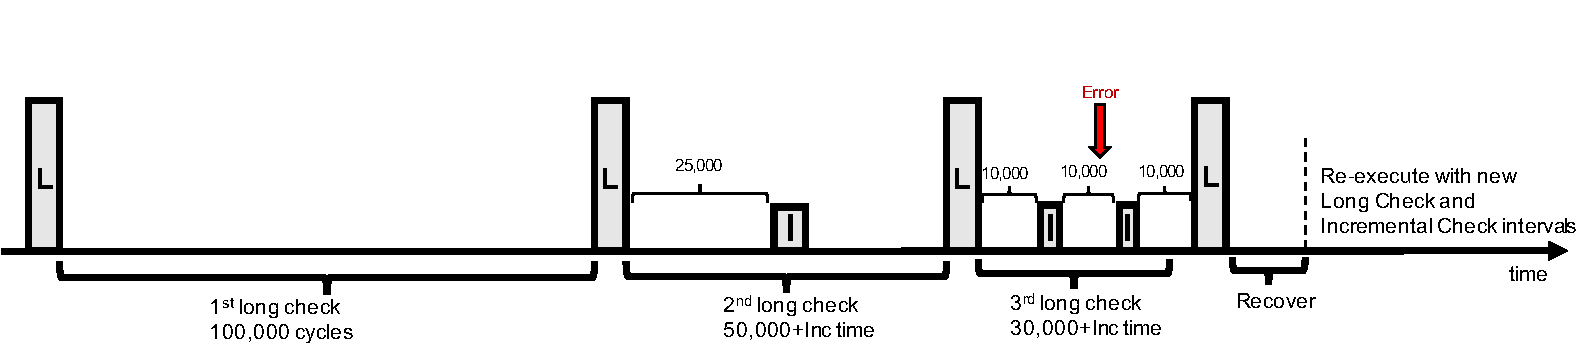
\includegraphics[width=3.3in]{graphics/adaptive21.pdf}%
\label{fig_adp_21}}
\caption{Error Interval Heuristics(EIH) Mechanism Examples}
\label{fig_adp_2}
\end{figure*}

%\begin{table}[h]
%  \caption{Formatting guidelines for submission.}
%  \centering
%  \begin{tabular}{|l|l|}
%    \hline
%    \textbf{Field} & \textbf{Value}\\
%    \hline
%    \hline
%    File format & PDF \\
%    \hline
%    Page limit & 11 pages, {\bf not including}\\
%               & {\bf references}\\
%    \hline
%    Paper size & US Letter 8.5in $\times$ 11in\\
%    \hline
%    Top margin & 0.75in\\
%    \hline
%    Bottom margin & 1in\\
%    \hline
%    Left margin & 0.75in\\
%    \hline
%    Right margin & 0.75in\\
%    \hline
%    Body & 2-column, single-spaced\\
%    \hline
%    Space between columns & 0.25in\\
%    \hline
%    Body font & 10pt\\
%    \hline
%    Abstract font & 9pt, bold\\
%    \hline
%    Section heading font & 12pt, bold\\
%    \hline
%    Subsection heading font & 10pt, bold\\
%    \hline
%    Caption font & 9pt (minimum)\\
%    \hline
%    References & 8pt, no page limit, list \\
%               & all authors' names\\
%    \hline
%  \end{tabular}
%  \label{table:formatting}
%\end{table}


%------------------------------------------------



%\vspace{-1mm}
%\begin{figure}[H]
%\begin{centering}
%\setlength{\abovecaptionskip}{-1mm} 
%\setlength{\belowcaptionskip}{-3mm} 
%\includegraphics[width=0.5\textwidth]{graphics/MMRcomp.pdf}
%\protect\caption{\label{fig:ComplementMMR}Complement M*MR signed representation}
%\par\end{centering}
%\vspace{-2mm}
%\end{figure}


% An example of a floating figure using the graphicx package.
% Note that \label must occur AFTER (or within) \caption.
% For figures, \caption should occur after the \includegraphics.
% Note that IEEEtran v1.7 and later has special internal code that
% is designed to preserve the operation of \label within \caption
% even when the captionsoff option is in effect. However, because
% of issues like this, it may be the safest practice to put all your
% \label just after \caption rather than within \caption{}.
%
% Reminder: the "draftcls" or "draftclsnofoot", not "draft", class
% option should be used if it is desired that the figures are to be
% displayed while in draft mode.
%
\section{Evaluation Methodology}
\label{sec:eval}
To measure the performance-energy-reliability trade-off of different RRNS cores, we augment a stochastic fault injection mechanism into a cycle-accurate in-order trace-based simulator. We abstract the notion of using next-generation devices operating at low signal energies ($E_s$) and the resulting interaction with the $kT$ noise floor into $P_e$, the probability of an error occurring in a transistor state in any given cycle. $E_s$, provided as one of the input to the simulation, is a measure of the signal energy at the input of a transistor; $P_e$ is the probability of a fault occurring at the output of a transistor in any given cycle. The relationship of $E_s$ and $P_e$ can be defined by the following equation: $P_e = exp( \frac{-E_s}{kT})$. Similar to the CREEPY simulator\cite{DengICRC16,DengTACO18}, these inputs are vectors as they denote the signal energies and error probabilities for each voltage domain, however, for the simple explanation purposes, we present them as scalars in the remainder of this section. Also input to the simulator is the check insertion strategy. The RRNS check could be placed in static or adaptive methods. Because we are evaluating a very different number system, we simulated an unpipelined microarchitecture with no branch prediction and a 2-level memory hierarchy (LLC-DRAM, with latencies of 12 cycles and 100 cycles for LLC hit and miss respectively) to maintain our primary focus in this paper. Adding more memory features to our design has been left as future work.

We first introduce a series of error events and their probabilities.
\begin{description}
\item[$P_e$] 
Probability of an error occurring in a transistor state in any given cycle. This is provided as an input to the simulation, as just discussed.

\item[$P_{add}$]
Probability of at least a single error in an adder (each sub-core has an adder in ALU). If there are $N_{add}$ transistors in an adder, the probability of each of these transistors being free of error is $(1-P_e)^{N_{add}}$. Therefore, $P_{add}$=1-$(1-P_e)^{N_{add}}$. Similarly, $P_{sub}$ and $P_{mul}$ are calculated. For multi-cycle operations, this definition holds as long as the state of each transistor is used exactly once for the operation. This is true for the said operators. Note that this is a conservative (pessimistic) estimate in our evaluation because we ignore any error masking that may potentially occur.

% TODO: Document (commented) derivation of transistor counts of all structures. This will help with rebuttal.

\item[$P_{R_i}$]
Probability of at least 1 error being present in a slice (sub-core/residue) of register $R_i$ since its last write. To compute this, we devise a $StateTable$, the $i^{th}$  entry of which holds the tuple ($P$, $cycle$), where, $P$ is the probability of $R_i$ having atleast 1 error being present in the corresponding residue upon its most recent update at cycle $cycle$. This $StateTable$ is updated for each register write. 

For example, consider the register $R_0$. 1) At cycle 0, the default value of $R_0$ tuple is ($P$=0, cycle=0). 2) At cycle 10, assume that we have an ADD instruction: ADD R0, R1, R2, and that it is the first instruction writing to $R_0$. We then update the tuple value to (Error\_Probability\_ADD, 10). It is necessary to update the $P$ value here because the error probability of this ADD instruction should be taken into account. $P$ value would then be set back to 0 once an RRNS check is inserted for that register and no error is detected, and then set the current system cycle value to the cycle field. This way, the $P$ field in the $StateTable$ always reflects the probability of that register of having at least 1 error being present in one of its residues, given its most recent update at the cycle field. 

Assuming an SRAM implementation of 8-bit wide $R_i$, the number of transistors is $8\times 6=48$. The probability of $R_i$ being error free is subject to two probabilities: (1) probability of an error-free write, ($P_1 = 1 - StateTable[R_i].P$) and, (2) probability of no error creeping into it since its last write ($P_2 = (1 - P_e')^{48(c - StateTable[R_i].cycle)}$), where, $c$ is the current cycle and $P_e'$ is the probability of an error occurring in the state of an SRAM transistor. Due to the nature of an SRAM device, any fault occurring in one of its transistors gets latched, resulting in a higher probability of an error (when compared with glitches in logic transistors getting masked if the glitch does not occur close to the clock edge). As such, we assume $P_e'=100P_e$. Putting it all together, we have $P_{R_i} = 1 - P_1*P_2$.

\item[$P_{LOAD ~X}$]
Probability of at least 1 error being present in the loaded data of address $X$. This is analogous to $P_{R_i}$, with the extended $StateTable$ storing an entry for each cache line. As we assume a perfect off-chip (ECC protected) main memory, cache miss repairs are initialized with a zero probability in error, and cache replacement victims' entries are also evicted from the $StateTable$. Finally, $P_{LOAD~X}$ encapsulates the probability of an error in the implicit computation of the address $X$ itself (from its base and offset) during the execution of the load, in addition to the probability of an error in the loaded data from the cache line.

\item[$P_{SC}$]
Probability of at least 1 error occurring in a sub-core from the last time it was checked. To illustrate, consider the following add instruction: $ADD~R_3,R_2,R_1$. Then, at the end of instruction, $P_{SC}=1-(1-P_{add})(1-P_{R_2})(1-P_{R1})$.

\item[$P_C^{1}$]
Probability of exactly 1 error occurring in a RRNS core from the last time it was checked. This translates to exactly 1 sub-core being in error (where the sub-core error itself may be of multi-bit form; RRNS can tolerate multi-bit flips within a single residue). Therefore, $P_C=6C_1\times P_{SC}(1-P_{SC})^5$, where the combinatorial choose operator $nC_r$ enumerates the number of ways in which $r$ items can be chosen from $n$ distinct items.

\item[$P_C^{0}$]
Probability of no error in a RRNS core from the last time it was checked. $P_C^{0}=6C_0 \times (1-P_{SC})^6 = (1-P_{SC})^6$.

\item[$P_C^{fail}$]
Probability of a RRNS core failing at any given cycle, since the last time it was checked. The current version of the RRNS checkpoint micro-architecture could detects one or two errors. For the (4,1)-RRNS version, we deem $\geq 2$ errors in the core as amounting to a failure. Therefore, $P_C^{fail}=\sum_{2\leq r\leq 6} 6C_r\times P_{SC}^r(1-P_{SC})^{6-r}=1-P_C^0-P_C^1$.  Similarly, for the (4,2)-RRNS version, we deem $\geq 3$ errors in the core as amounting to a failure. Therefore, $P_C^{fail}=1-P_C^0-P_C^1-P_C^2$. 

\end{description}

Note that the computation of these error probabilities is done after every instruction (irrespective of the check insertion strategy) for the purposes of bookkeeping such as $StateTable$ update and to estimate the probability of a failure $P_{C, i}^{fail}$ at each time step $t_i$. We use a typically used reliability metric, Mean Time Between Failure (MTBF) \cite{tan2004process}, which can be defined as follows: $MTBF=\frac{Total~Cycles}{CPU~Frequency~\times~\sum_iP_{C, i}^{fail}}$. The subscript \textit{i} in $P_{C, i}^{fail}$ represents the ${i}^{th}$ instruction of the instruction stream. MTBF also corresponds to mean time to checkpoint recovery. 


\section{EXPERIMENTAL EVALUATION}
\label{Evaluation}

\subsection{Minimal Signal Energy with Reasonable Reliability}
\label{sub:SignalEnergy}
The lowest signal energy values of normal logic in (4,2)-RRNS Single Error Correction(SEC) system are range from 28-31KT\cite{DengTACO18}. In theory, the related signal energy values could be further turn down by adopting the (4,2)-RRNS Double Error Detectction(DED) configuration. The DED system equips with stronger error detection and recovery ability and only the cases of 3 or more errors are defined as failure. So this give the potential of signal energy goes down further. 

In order to figure out the optimal signal energy of normal logic in energy and Energy Delay Product(EDP), we design 3 signal energy experiments with fixed 100K-cycle long time interval and 10K-cycle incremental interval.  Figure \ref{SignalE} gives the MTBF values with signal energy between 16KT to 23KT. The MTBF is defined as 'Reasonable' only if the value is equal or larger than 100 years. From this figure we can reach a conclusion that the minimal signal energy is 17KT to meet the reliability requirement. Figure \ref{SignalE1} shows the normalized energy values with signal energy between 17KT-23KT. The energy consumption of 23KT configurations are normalized to 1. If the signal energy is equal or less than 17KT, the energy overhead increase dramatically due to error rate raise. The minimal energy values are detected when the signal energy is set to 18 or 19 KT, depending on the specific workload. Similarly,  Figure \ref{SignalE2} demonstrates we can get the optimal EDP if the signal energy is set to 18 or 19 KT. Based on these 3 figures, the signal energy could be further turned down to 18-19 KT for (4,2)-RRNS DED configuration, which is much lower than 28-31KT in (4,2)-RRNS Single Error Correction(SEC) system. So the checkpoint and rollback method has the potential to beat the correction scheme. 18 or 19 KT is used in the following experiments for (4,2)-RRNS general logic when making the comparison with other cores. 

\begin{figure*}[!t]
\centering
\subfloat[Minimal MTBF Values]{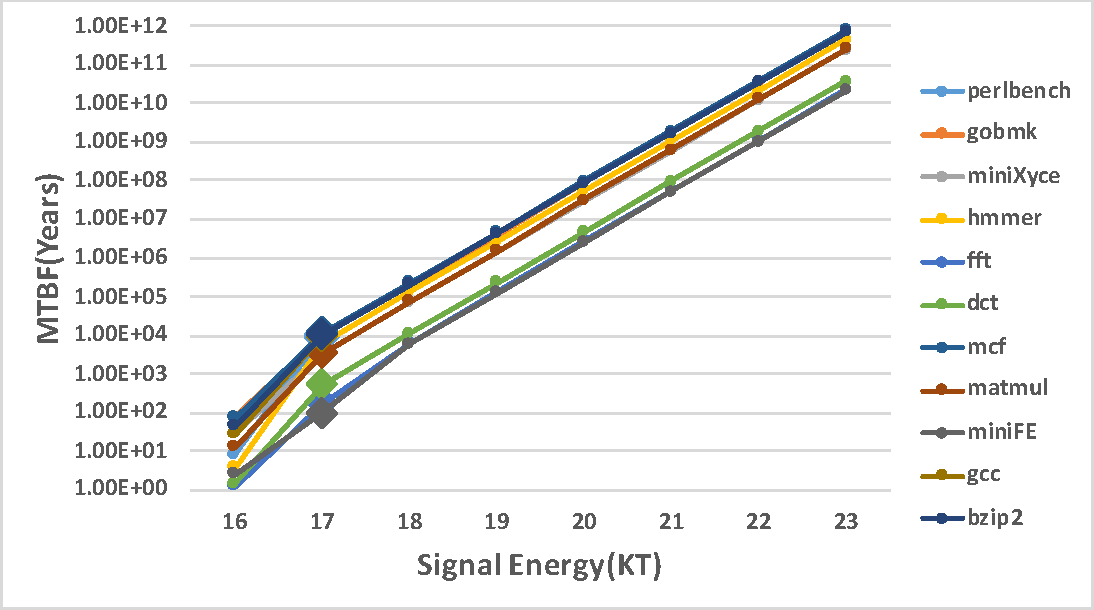
\includegraphics[width=2.3in]{graphics/SignalE.pdf}%
\label{SignalE}}
\hfil
\subfloat[Minimal Energy Values]{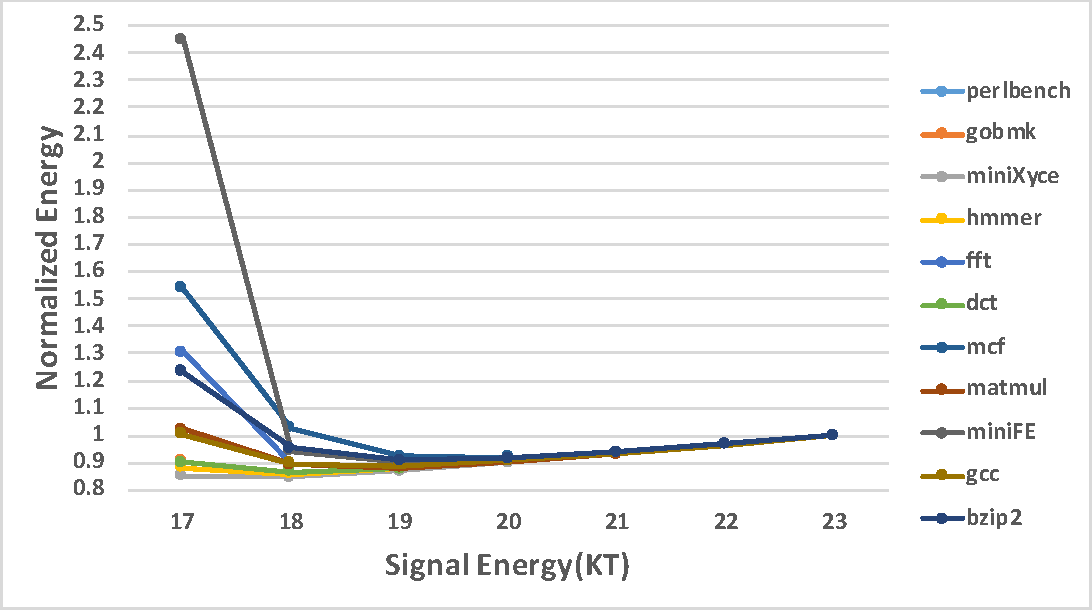
\includegraphics[width=2.3in]{graphics/SignalE1.pdf}%
\label{SignalE1}}
\hfil
\subfloat[Minimal EDP Values]{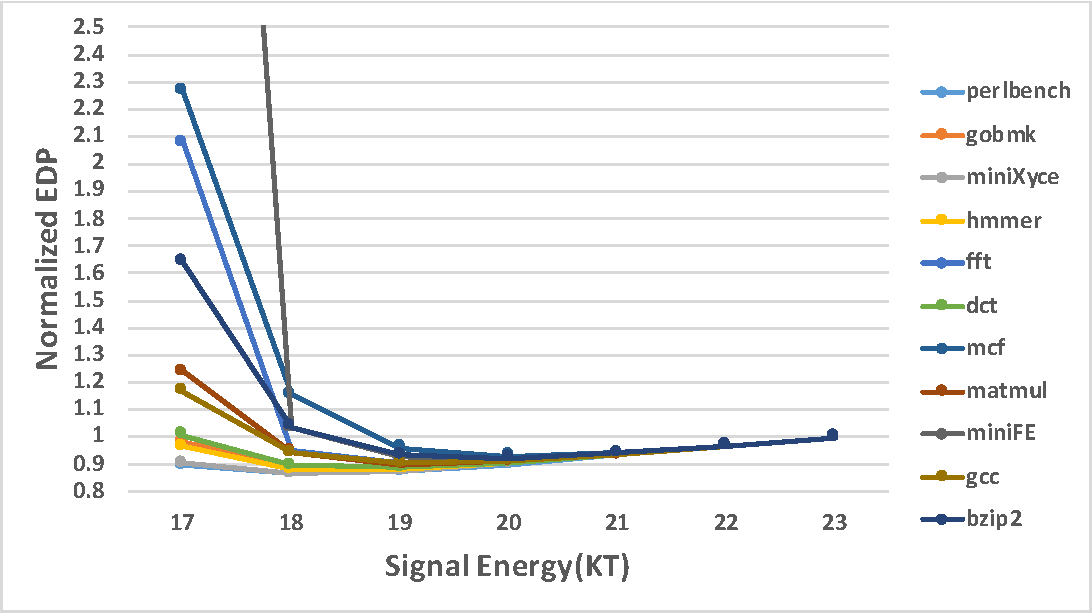
\includegraphics[width=2.3in]{graphics/SignalE2.pdf}%
\label{SignalE2}}
\caption{Minimal Signal Energy Of Normal Logics For All The Workloads}
\label{fig_sim}
\end{figure*}


\subsection{Energy Delay Product(EDP) Comparison of 3 RRNS Configurations}
\label{sec:3Config}
The potential of energy and EDP reduction has been verified in Section \ref{sub:SignalEnergy}. However, figuring out how much optimization it can be achieved is also necessary. Figure \ref{fig_41RRNS} shows the Energy Delay Product(EDP) comparison of (4,2)-RRNS Single Error Correction(SEC, CREEPY), (4,1)-RRNS Single Error Detection(SED) and (4,2)-RRNS Double Error Detectcion(DED). And the EDPs of CREEPY are normalized to 1. For the (4,2)-RRNS DED, we used static checkpoint scheme with 40 different configurations for each of workloads. The `\textit{static}' means both \textit{long\_check\_interval} and \textit{incremental\_interval} are stable during the execution. In these 40 configurations, the long check intervals are range from 1K to 500K cycles while the incremental intervals are set from 1K to 100K cycles. The \textit{incremental\_intervals} are always less than or equal to  \textit{long\_check\_interval}. The (4,2)-RRNS-static-ave in the figure represents the arithmetic average of the 40 results.  

(4,1)-RRNS SED is worst in all the workloads even though it uses less subcore hardware and RIU consistent check logics. The primary reason of this counterintuitive phenomenon is  (4,1)-RRNS SED loss reliability while trying to reduce the energy consumption in normal computation and checking. On average, one third of errors are undetectable in (4,1)-RRNS SED and this could explain the system MTBFs decreasing. In order to make a fair comparison of all the proposed RRNS configurations, we set the signal energy values and keep the related MTBFs to a same level(Larger or equal to 100 years). In the (4,1)-RRNS SED, we have to use higher single energy to keep the reliability(41-42KT in (4,1)-RRNS SED; 28-31KT in ((4,2)-RRNS SEC); 18-19KT in (4,2)-RRNS DED).  Because of the good error detection ability in (4,2)-RRNS DED, it gets the best EDP in this comparison. Failure only occurs when two or more residues are in error. 3 or more residues in error may also detectable in some cases(discussed in previous section?). Because only the static checkpoint scheme is used in this section, the potential of more energy and EDP reduction may be achieved if designing some reasonable adaptive checkpoint and rollback methods.  

\begin{figure}[H]
\centering
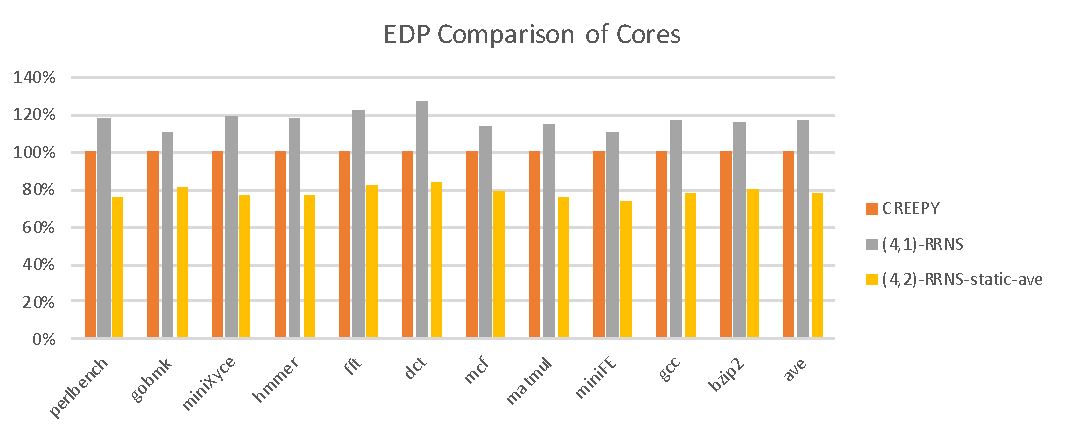
\includegraphics[width=3.5in]{graphics/41RRNS.pdf}
\caption{EDP Comparison of Cores}
\label{fig_41RRNS}
\end{figure}

\subsection{Energy Breakdown of Static-best Checkpoint Configurations}
Figure \ref{fig_Energybreakdown} lists the extra overhead breakdowns of the best static checkpoint configurations for each of the workloads. The `\textit{best}' represents the optimal EDP in 40 configurations. These extra energy overhead are defined into four types: 1) The energy overhead of creating the incremental checkpoints; 2) The energy overhead of all full checkpoint verifications, which operate at the end of every long check interval; 3) Re-execution overhead after system state recovery; 4) Extra recovery energy once the error is detected, and this includes the full checkpoint status and incremental checkpoint status recovery. From the result, the extra energy overhead is low in majority of the workloads. Except gobmk, all the other energy overhead values are less than 6\%, which means the static-best configurations do well in energy saving and the potential of adaptive method improvement is limited when comparing with it. But a big problem of static-best is we are difficult to figure out which static checkpoint configuration(value pair of  \textit{long\_check\_interval} and \textit{incremental\_interval}) is best for a specific benchmark. We found the best static configuration always vary in different workloads. So efficient adaptive checkpoint methods are still necessary even though they may be no significant improvement when comparing with the best-static checkpoint configuration. 

\begin{figure}[H]
\centering
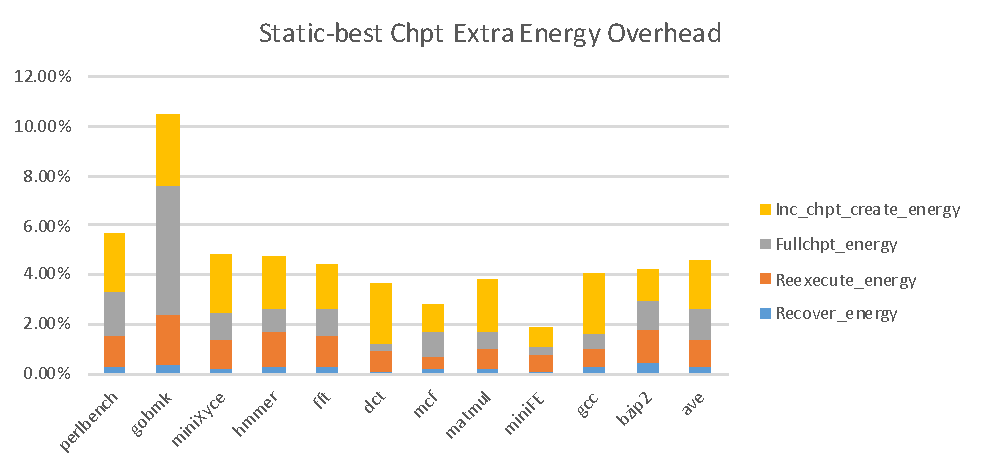
\includegraphics[width=3.5in]{graphics/Energybreakdown.pdf}

\caption{Extra Energy Overhead Breakdown of Static-best Checkpoint Configurations}
\label{fig_Energybreakdown}
\end{figure}

\subsection{Energy and EDP Comparison}
% Note that the IEEE typically puts floats only at the top, even when this
% results in a large percentage of a column being occupied by floats.
Energy is the primary consideration for extending the Denard scaling \cite{Dennard}. Figure \ref{fig_first_case} compares the energy consumption of all the proposed checkpoint schemes. And the energy consumption of CREEPY, which implements as (4,2)-RRNS Single Error Correction(SEC), is normalized as 1. Because (4,1)-RRNS SED was demonstrated worse than CREEPY in Section \ref{sec:3Config}, in this figure we only focus on (4,2)-RRNS Double Error Detection(DED). Static-ave is the average energy values of 40 different static checkpoint point evaluations with the long check intervals vary from 1K to 500K cycles while the incremental intervals are set from 1K to 100K cycles. And Static-best the picks the lowest energy consumption configuration. It should be noted that the related best configuration is inconsistent among the different workloads. In reality it should be hard to get the excellent energy reduction if  randomly picking a checkpoint configuration. In other words, the Static-best is hard to achieve in practice. For the Extra Overhead Estimation(EOE) adaptive method, it better than Static-ave in all the benchmarks and worse than Static-best in most cases. The Error Interval Heuristics(EIH) method is always best in all workloads. On average, it gets 31.79\%,  8.99\%,  1.24\% energy reduction respectively when comparing with CREEPY, Static-ave and Static-best. For the EDP comparison in Figure \ref{fig_second_case}, we can get a similar conclusion, EIH adaptive checking method gets the best EDP and EOE is a little worse than Static-best. The energy and EDP reductions of EIH are not significant when comparing with Static-best. The reason of this limit improvement could be explained in Figure \ref{fig_Energybreakdown}. The extra overhead of Static-best is less than 6\% in most cases, so the improvement should be constrained to this upper bound. Moreover, the Static-best is always hard to figure out unless running the application multiple times. 
% An example of a double column floating figure using two subfigures.
% (The subfig.sty package must be loaded for this to work.)
% The subfigure \label commands are set within each subfloat command,
% and the \label for the overall figure must come after \caption.
% \hfil is used as a separator to get equal spacing.
% Watch out that the combined width of all the subfigures on a
% line do not exceed the text width or a line break will occur.
%
\begin{figure*}[!t]
\centering
\subfloat[Energy]{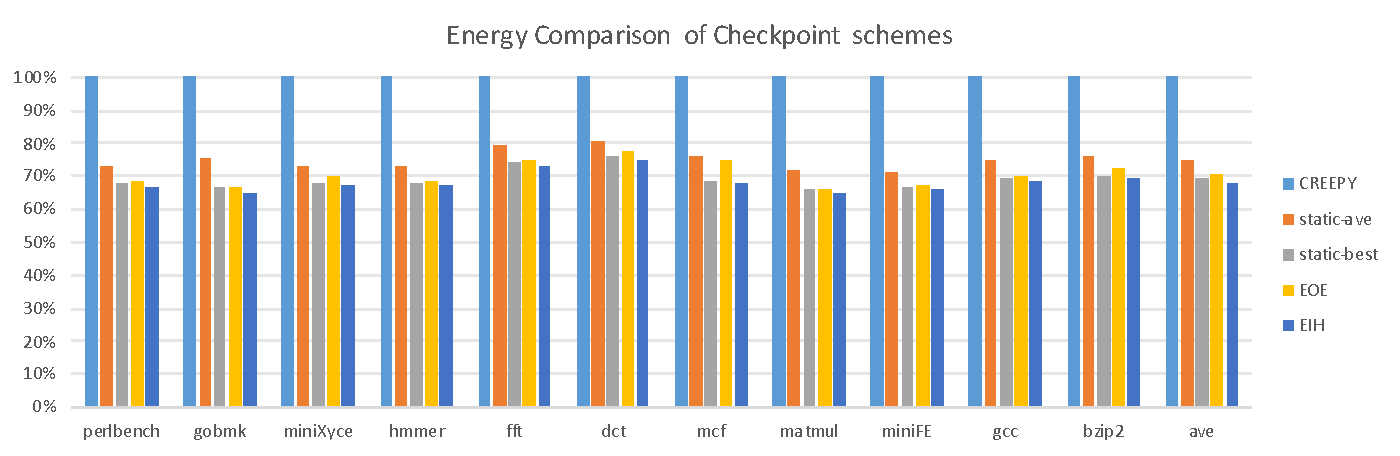
\includegraphics[width=3.2in]{graphics/energy.pdf}%
\label{fig_first_case}}
\hfil
\subfloat[Energy Delay Product(EDP)]{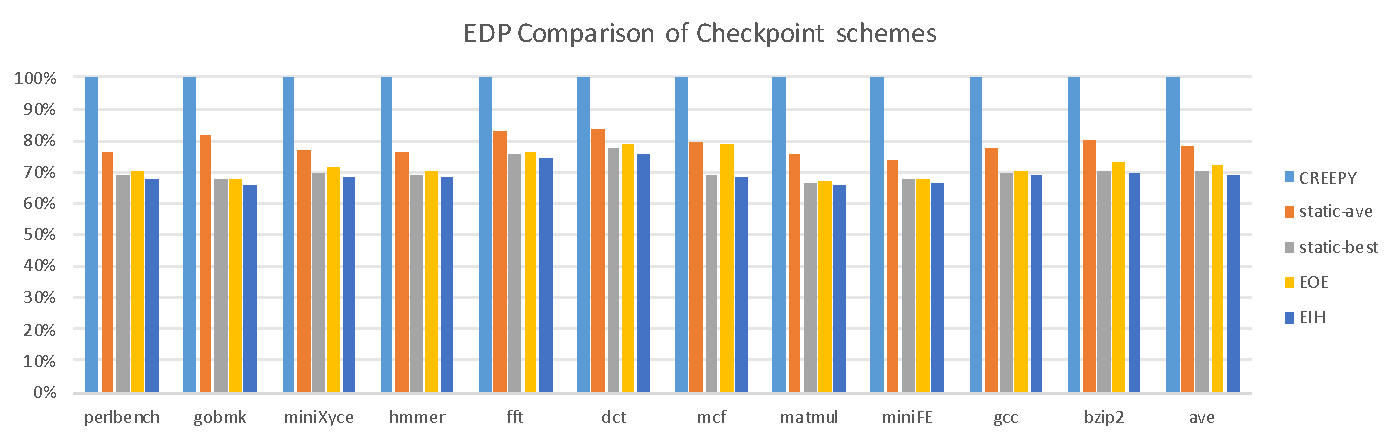
\includegraphics[width=3.2in]{graphics/EDP.pdf}%
\label{fig_second_case}}
\caption{Comparison of Checkpoint Schemes}
\label{fig_sim}
\end{figure*}
%
% Note that often IEEE papers with subfigures do not employ subfigure
% captions (using the optional argument to \subfloat[]), but instead will
% reference/describe all of them (a), (b), etc., within the main caption.
% Be aware that for subfig.sty to generate the (a), (b), etc., subfigure
% labels, the optional argument to \subfloat must be present. If a
% subcaption is not desired, just leave its contents blank,
% e.g., \subfloat[].


% An example of a floating table. Note that, for IEEE style tables, the
% \caption command should come BEFORE the table and, given that table
% captions serve much like titles, are usually capitalized except for words
% such as a, an, and, as, at, but, by, for, in, nor, of, on, or, the, to
% and up, which are usually not capitalized unless they are the first or
% last word of the caption. Table text will default to \footnotesize as
% the IEEE normally uses this smaller font for tables.
% The \label must come after \caption as always.
%
%\begin{table}[!t]
%% increase table row spacing, adjust to taste
%\renewcommand{\arraystretch}{1.3}
% if using array.sty, it might be a good idea to tweak the value of
% \extrarowheight as needed to properly center the text within the cells
%\caption{An Example of a Table}
%\label{table_example}
%\centering
%% Some packages, such as MDW tools, offer better commands for making tables
%% than the plain LaTeX2e tabular which is used here.
%\begin{tabular}{|c||c|}
%\hline
%One & Two\\
%\hline
%Three & Four\\
%\hline
%\end{tabular}
%\end{table}


% Note that the IEEE does not put floats in the very first column
% - or typically anywhere on the first page for that matter. Also,
% in-text middle ("here") positioning is typically not used, but it
% is allowed and encouraged for Computer Society conferences (but
% not Computer Society journals). Most IEEE journals/conferences use
% top floats exclusively.
% Note that, LaTeX2e, unlike IEEE journals/conferences, places
% footnotes above bottom floats. This can be corrected via the
% \fnbelowfloat command of the stfloats package.




%\section{Conclusion}
%The conclusion goes here.




% conference papers do not normally have an appendix


% use section* for acknowledgment
\section{Related Work}
\label{sec:related}

\textbf{RNS and RRNS}
The energy efficient properties of RNS due to its low-bit-width operations and absence of carries across residues has found applications in the digital signal processing (DSP) \cite{Chokshi,Claudio,Ramirez} domain. Furthermore, the representability of high bit-width integers as a tuple-of-resides has been leveraged by the cryptography (RSA) \cite{bajard2004RSA,hung1994RSA,yen2003RSA} community. Anderson~\cite{AndersonThesis} proposed an architecture and ISA for an RNS co-processor designed to run datapath operations in tandem with a general-purpose processor running binary instructions, where the primary role of the general purpose processor is to handle control flow. The RNS co-processor uses an accumulator based ALU and does not support caching or computational error correction (RRNS). Furthermore, it requires a conversion to binary (and vice-versa) for comparison operations, which is expensive. Deng etc.\cite{DengTACO18} proposed a Single Error Correction RRNS core (CREEPY) with ISA is significantly more efficient. However, due to it can only detect one residue in error, the reliability and this architecture is limited and the signal energy of transistor could be further turn down. In other words, CREEPY is not the energy lower bound. 

Chiang et al. \cite{JSHIUN_FP} provide RNS algorithms for comparison and overflow detection, but assume all bases to be odd and do not consider error correction. Similarly, Preethy et al. \cite{preethy1999,preethy2000rns} integrate index-sum multiplication into RNS, but do not consider its impact on the properties of RRNS bases critical to RRNS checkpoint  and rollback system.

Ever since Watson and Hastings \cite{Hastings,WatsonThesis,WatsonHastings} introduced RRNS as an efficient means for computational error correction, there has been a significant body of research \cite{tay2016non,bajard2016multi,xiao2016new,xiao2015error,chang2015residue,tay2014new,yin2013new,lo2013parallel,sengupta2013performance,haron2011redundant,tang2010new,goh2008multiple,sweidan2001theory,goldreich1999chinese,katti1996new,krishna1994computational,di1993systolic,krishna1992coding,sun1992coding,sun1992superfast,orton1992new,su1990algorithm,ramachandran1983single,etzel1980redundant,barsi1974error,yau1973error,rao1970biresidue,szabo1967residue} that strives to improve upon it. These are orthogonal to our checkpoint  architeture, and further such algorithmic research can be used to optimize aspects of the core itself, such as the RIU.

\textbf{Computational Error Correction}

\begin{figure}[H]
\begin{center}
\setlength{\abovecaptionskip}{-0.2mm} 
%\setlength{\belowcaptionskip}{-0.5mm} 
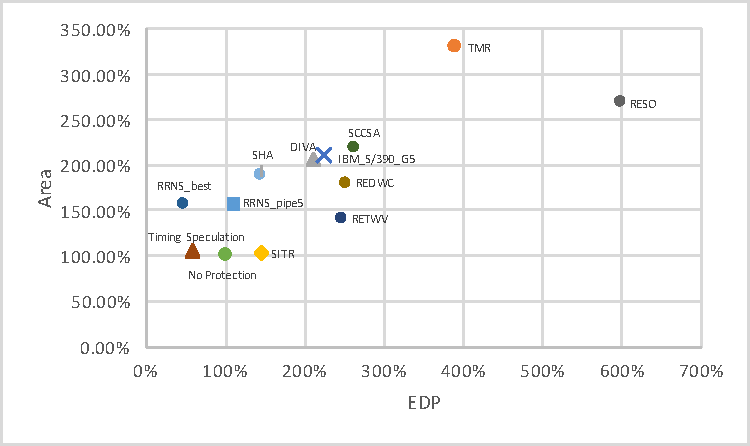
\includegraphics[width=3.25in,height=1.75in]{graphics/RelatedComp.pdf}
\\
\scriptsize{RESO\cite{RESO}, REDWC\cite{REDWC}, RETWV\cite{RETWV}, SCCSA\cite{SCCSA}, SHA\cite{SHA}, DIVA\cite{DIVA}, SITR\cite{SITR}, Timing Speculation\cite{razor_2003,decor_2008}}
%\vspace{-1mm}
\caption{First order comparison of area overhead and energy-delay product (EDP) of various mechanisms for computational error correction, depicting the superiority of RRNS. Computational error correction techniques use a combination of spatial and temporal redundancy techniques. While temporal redundancy allows for a low area overhead, they suffer from a significant performance penalty. Timing speculation techniques seem more efficient than RRNS, however, their error model assumes all bit errors manifest as circuit timing errors, which is not sufficient to work with ultra low energy logic devices.}
\label{fig:related}
\end{center}
\vspace{-3mm}
\end{figure}

Standard error correcting codes (ECC)\cite{macwilliams1977theory} have already been adopted into modern memory systems. These codes accommodate errors occurring in storage and communication/network traffic, but are not able to protect computational logic. The naive approach to computational error correction is triple modular redundancy (TMR)\cite{von1956probabilistic}, requiring over a 200\% overhead in area and energy for single error correcting capability. Several techniques in the form of arithmetic codes such as AN codes\cite{brown1960error,fetzer2009encoding,forin1989vital,liu1972error,schiffel2010anb,wappler2007hardware}, self-checking\cite{johnson1988efficient,keren2008arbitrary,marienfeld2005new,nicolaidis2003carry,nicolaidis1998design,nicolaidis1994efficient,vasudevan2005technique} and self-correcting\cite{sun2010cost,hsu1992time,peng2005fault,dolev2013preserving,ghosh2008novel,krekhov2008method,mathew2010multiple,rao2008towards,rao2006fault,valinataj2007fault} adders and multipliers have since been devised. Orthogonally, proposals employ redundancy at a higher granularity, such as timing speculation (wherein error correction capability is limited to circuit timing violations)\cite{razor_2003,decor_2008}, partial pipeline replication\cite{DIVA} or checkpoint-rollback-recovery such as those in IBM Power8 processors\cite{ibmpower8}. While these are more efficient than naive TMR, they come with limitations on their error model, or, their area overheads are still over 100\% and/or incur a significant performance penalty, owing to the fact that they leverage temporal redundancy in an effort to minimize area overhead\cite{srikanth2016brief}

Figure \ref{fig:related} summarizes some of these techniques in comparison with RRNS. We refer the interested reader to Srikanth et al.\cite{srikanth2016brief} for a more detailed survey on some of these non-residue techniques, but the takeaway is that RRNS is generally considered superior in terms of capability and efficiency for computational error resilience. 

Approaches that employ timing speculation\cite{razor_2003,decor_2008} may seem superior to RRNS at first glance. However, the error model that can be supported by an RRNS error correcting microarchitecture is orthogonal to theirs, if not broader. For example, razor\cite{razor_2003} uses conventional transistors, therefore lowering $V_{dd}$ lowers MOSFET switching speed, resulting in a frequency drop, which could cause setup time violations that they handle via a delayed latch mechanism. They assume that any error manifests itself as a timing error. Similarly, decor\cite{decor_2008} uses a delayed commit approach (with rollback support) to handle violations in timing margins. However, with emerging devices (Section \ref{sec:intro}), $V_{dd}$ can be lowered to few tens of millivolts without frequency loss, meaning that operating at the resultant thermal noise floor leads to \textit{stochastic, intermittent} bit flips, which cannot be captured as circuit timing errors. Unlike such approaches, a RRNS core with checkpoint mechanism can not only tolerate such errors in the data path, but also in the control path between memory accesses.

In terms of being able to tolerate control path errors, approaches such as DIVA\cite{DIVA} that replicate parts of the pipeline are capable. Their design provides recovery by having a simple core recalculate results of an out-of-order core. In this approach, the simple core is assumed to be error-free.  This is similar to a "double-modular-redundancy" approach with a rad-hard node, implying a relatively high overhead. Furthermore, if the rad-hard simple core is instead prone to error, checkpoint and re-execute methods would need to be employed, similar to the IBM POWER7/8 processors\cite{ibmpower8}. On the other hand, a RRNS core is able to tolerate errors in its redundant as well as non-redundant computations.

\section{Conclusion}
The upcoming next generation device such as tunneling FETs and ferroelectric/negative- capacitance FETs enables reduction of supply voltage to few tens of millivolts without degradation in switching speed. However, as a result of operating close the the kT noise  floor, computational logic is subject to intermittent, stochastic errors.  The RRNS representation is a promising approach towards using such ultra low power devices, by employing efficient computational error correction or detection with checkpoint.
In this paper, we design (4,1)-RRNS and (4,2)-RRNS checkpoint systems with reasonable base sets and supported incremental checkpoint mechanism. By using the RRNS checkpoint and rollback mechanism, we can safely remove a ROM unit which stored the large size error correction table. We also verified that (4,2)-RRNS DED configuration could further reduce energy and EDP while (4,1)-RRNS SED doesn't. Finally we proposed 2 adaptive checkpoint interval adjustment methods and reducing 31.79\% in energy consumption and 31.1\% in EDP when comparing with the previous single error correction architecture (CREEPY). 

\section*{Acknowledgements}
We thank the anonymous reviewers of the review process for their constructive feedback on this research.



% trigger a \newpage just before the given reference
% number - used to balance the columns on the last page
% adjust value as needed - may need to be readjusted if
% the document is modified later
%\IEEEtriggeratref{8}
% The "triggered" command can be changed if desired:
%\IEEEtriggercmd{\enlargethispage{-5in}}

% references section

% can use a bibliography generated by BibTeX as a .bbl file
% BibTeX documentation can be easily obtained at:
% http://mirror.ctan.org/biblio/bibtex/contrib/doc/
% The IEEEtran BibTeX style support page is at:
% http://www.michaelshell.org/tex/ieeetran/bibtex/
%\bibliographystyle{IEEEtran}
% argument is your BibTeX string definitions and bibliography database(s)
%\bibliography{IEEEabrv,../bib/paper}
%
% <OR> manually copy in the resultant .bbl file
% set second argument of \begin to the number of references
% (used to reserve space for the reference number labels box)
%\begin{thebibliography}{1}
%
%\bibitem{IEEEhowto:kopka}
%H.~Kopka and P.~W. Daly, \emph{A Guide to \LaTeX}, 3rd~ed.\hskip 1em plus
%  0.5em minus 0.4em\relax Harlow, England: Addison-Wesley, 1999.
%
%\end{thebibliography}


\bibliographystyle{IEEEtran.bst}
\bibliography{ref}

\appendix

  \subsection{Expected Error Time in EOE Adaptive Checking}
  \label{appendix}
The expected error time in the last long check interval could be defined as follow: 

  \scriptsize 
  \begin{spacing}{0.8}
  \textit{\[E(X) =\lim_{\substack{N\to \infty}}\frac{\text{Sum of  Error  Cycles  in  N  Experiments}}{\text{Num  of  Errors  in  N  Experiments}}\]}
\[=\lim_{\substack{N\to \infty}}\frac{N*(1*P_{1}+2*P_{2}+3*P_{3}...+L*P_{L})}{N*(P_{1}+P_{2}+P_{3}...+P_{L})}\]
  \end{spacing}
  \[=\frac{(1*P_{1}+2*P_{2}+3*P_{3}...+L*P_{L})}{(P_{1}+P_{2}+P_{3}...+P_{L})} \hspace{1cm}(1)\] 
 \normalsize
  \begin{spacing}{1}
\textbf{ $P_{i}$} in Formula (1) represents the the error is detected in the \textbf{ $i_{th}$}  cycle of the last long interval and  \textbf{ $P_{i} =  {A(1-A)}^{i-1}$}. We assume the system issues a load instruction in every cycle and make the expected value estimation in a simple way. So we have
\end{spacing} 
\scriptsize 
 \begin{spacing}{0.8}
 \[A= 1-{(1-{P}_{err\_sram\_t})}^{TCount}\] 
 \end{spacing} 
  \normalsize
  \begin{spacing}{1}
 \textit{ ${P}_{err\_sram\_t}$} represents the fault probability of a single SRAM transistor and  \textit{TCount} is the active SRAM transistor number of the load operation. So we get a new format of formula (1):
\end{spacing}
  \scriptsize 
   \begin{spacing}{0.8}
  \[E(X)=\frac{\sum_{i=1}^{L} i*A{(1-A)}^{i-1}}{\sum_{i=1}^{L} A{(1-A)}^{i-1}} \hspace{1cm}(2)\] 
  \end{spacing} 
 \normalsize
For the denominator of Formula (2):
 \scriptsize
  \begin{spacing}{0.6}
   \[\sum_{i=1}^{L} A{(1-A)}^{i-1} = \sum_{i=1}^{L} {(1-A)}^{i-1} - \sum_{i=1}^{L} {(1-A)}^{i}\] 
   \[=  \frac{1-(1-A)^{L}}{1-(1-A)} - \frac{(1-A)(1-(1-A)^L)}{1-(1-A)}\] 
  \end{spacing}
\[=  \frac{(1-A)^{L+1} - (1-A)^{L} +A}{A} \hspace{1cm}(3)\] 
  \normalsize
   \begin{spacing}{0.8}
  Similarly, for the numerator of Formula (2):
  \end{spacing}
  \scriptsize
  %\begin{spacing}{0.6}
\[\sum_{i=1}^{L} i*A{(1-A)}^{i-1} = \sum_{i=1}^{L} {i*(1-A)}^{i-1} - \sum_{i=1}^{L} {i*(1-A)}^{i}  \hspace{0.4cm}(4)\] 
 % \end{spacing}
  \normalsize
 \begin{spacing}{0.6}
Define a variable T: 
  \end{spacing}
\scriptsize 
%\begin{spacing}{0.6}
  \[T = \sum_{i=1}^{L} i*{(1-A)}^{i} = (1-A)+ 2(1-A)^2+\cdots+ L(1-A)^L\hspace{0.4cm}(5)\] 
%\end{spacing}
\normalsize
 \begin{spacing}{0.6}
And then multiply  \textit{(1-A)} in both sides of Formula (5):
  \end{spacing}
  \scriptsize 
  \[ \hspace{0.2cm} (1-A)T = (1-A)^2+ 2(1-A)^3+\cdots+ L(1-A)^{L+1}\hspace{0.4cm}(6)\] 
  \normalsize
 \begin{spacing}{1}
Formula (5) subtracts Formula (6):
  \end{spacing}
   \scriptsize 
  \[T- (1-A)T = (1-A)+ (1-A)^2+\cdots+ (1-A)^L - L(1-A)^{L+1}\] 
  \[= \frac{1-A-(1-A)^{L+1}}{A}- L(1-A)^{L+1}\hspace{0.4cm}(7)\] 
  \normalsize
 \begin{spacing}{1}
From Formula (7), we can compute the value of T:
  \end{spacing}
   \scriptsize 
    \begin{spacing}{0.6}
  \[T = \frac{1}{1-(1-A)}*(\frac{1-A-(1-A)^(L+1)}{A} - L(1-A)^{L+1})\] 
  \[ = \frac{1-A-(1-A)^{L+1}}{A^2} - \frac{L(1-A)^{L+1}}{A}\hspace{0.4cm}(8)\] 
   \[\therefore \textit{Formula (4)} = (\frac{1}{1-A}-1)*T = \frac{1-(1-A)^L}{A}- L(1-A)^L\hspace{0.4cm}(9)\] 
  \end{spacing}
   
  \normalsize
   \begin{spacing}{1.2}
Finally, we put Formula (3) and (9) into Formula (2), and get the value of E(X):
      \end{spacing}
   \scriptsize 
   \begin{spacing}{0.6}
  \[E(X) = (2) = [\frac{1-(1-A)^{L}}{A} - L(1-A)^L]*\frac{A}{(1-A)^{L+1} - (1-A)^L+A}\] 
  \[= \frac{1-(1-A)^L-AL(1-A)^L}{(1-A)^{L+1}-(1-A)^L+A}= \frac{1-(1+AL)(1-A)^L}{A-A(1-A)^L}  \hspace{1cm}(10)\] 
  \end{spacing}
  \normalsize


\end{document}
